\documentclass[spanish, c]{beamer}

\usepackage[utf8]{inputenc}
\usepackage[spanish, mexico]{babel}
\usepackage{amsmath}
\usepackage{mathtools}
\usepackage{hyperref}
\usepackage{xcolor}
\usepackage{color}
\usepackage{ragged2e}
\usepackage{mathrsfs}
\usepackage{csquotes}
\usepackage{listings}
\usepackage[scaled]{beramono}
\usepackage[T1]{fontenc}
\usepackage{matlab-prettifier}
\usepackage{graphicx}
\usepackage{booktabs}
\usepackage{tikz}
\usepackage{venndiagram}
\usepackage{semantic}

\renewcommand{\indent}{\hspace*{2em}}

% \usetikzlibrary{fit, shapes, arrows}

% \usepackage{courier}
% \usepackage{subfigure}
% \usepackage{enumerate}
% \usepackage{algorithmic}
% \usepackage{algorithm}

% \usepackage{listings}
% \usepackage{lstlinebgrd}

\usetheme{Boadilla}
\usefonttheme[onlymath]{serif}

\newcommand{\matlab}[1]{\lstinline[style=Matlab-editor]!#1!}
\newcommand\blfootnote[1]{%
\begingroup
\renewcommand\thefootnote{}\footnote{#1}%
\addtocounter{footnote}{-1}%
\endgroup
}

\lstset
{
    language = Matlab,
    style = Matlab-editor,
    basicstyle = \mlttfamily\scriptsize,
    escapechar = `,
    numbers = left,
    frame = tb,
}

\lstdefinestyle{output}
{
    language = {},
    basicstyle = \mlttfamily\scriptsize,
    escapechar = `,
    numbers = none,
    showtabs = false,
   	showstringspaces = false,
}

% Sets the templates
\definecolor{navyblue}{RGB}{0, 0, 128}
\definecolor{crimson}{RGB}{128, 16, 0}

\setbeamertemplate{navigation symbols}{}
\setbeamertemplate{headline}{}
\setbeamertemplate{title page}[default][colsep=-4bp,rounded=true]
\setbeamertemplate{footline}[frame number]
\setbeamertemplate{bibliography item}[text]
\setbeamertemplate{theorems}[numbered]

\setbeamercolor{title}{fg=navyblue, bg=white}
\setbeamercolor{frametitle}{fg=navyblue, bg=white}
\setbeamercolor{structure}{fg=navyblue}
\setbeamercolor{button}{fg=white,bg=navyblue}

\setbeamercovered{transparent}

\title{Conjuntos y Tablas Hash}
\subtitle{Programación de Estructuras de Datos y Algoritmos Fundamentales \\ (TC1031)}
\author{
    \texorpdfstring{
        \begin{center}
            M.C. Xavier Sánchez Díaz \\
            \href{mailto:mail@tec.mx}{\texttt{mail@tec.mx}}
        \end{center}
    }
    {M.C. Xavier Sánchez Díaz}
}

\institute[Tecnológico de Monterrey]{
\includegraphics[scale=0.5]{../img/logo}}
\date{}

\begin{document}

\setlength{\rightskip}{0pt}

\begin{frame}[plain]
    \titlepage        
\end{frame}

\begin{frame}{Outline}
    \tableofcontents
\end{frame}

\section{Revisión de Conjuntos}

\begin{frame}{¿Qué es un conjunto?}{Definición y propiedades de los conjuntos}

    Un \alert{conjunto} es un concepto abstracto, construido para referirse a una \textbf{colección} de \textbf{elementos}. \pause

    \bigskip

    Usualmente representamos los \alert{conjuntos} con letras mayúsculas (usualmente usando letras próximas a la $A$), y delimitamos sus contenidos con llaves (\textit{curly brackets}):

    \bigskip

    \begin{exampleblock}{Ejemplo}
        $A$ es el conjunto de los primeros cinco \textbf{números naturales}, es decir aquellos que \textit{nos sirven para contar}:
        $$A = \{1, 2, 3, 4, 5\}$$    
    \end{exampleblock}
\end{frame}

\begin{frame}{¿Qué es un conjunto?}{Definición y propiedades de los conjuntos}
    Un \textbf{conjunto} puede \alert{enumerarse} o \alert{describirse}:

    \bigskip

    \begin{exampleblock}{Enumeración o Extensión}
        $$A = \{1, 2, 3, 4, 5 \}$$
    \end{exampleblock}

    \bigskip

    \begin{exampleblock}{Descripción o Comprensión}
        \begin{itemize}
            \item $A = $ el conjunto de los primeros cinco números naturales
            \item $B = $ el conjunto de personas en este \textit{ZOOM Room}
            \item $C = $ el conjunto de estudiantes del Campus Monterrey
        \end{itemize}
    \end{exampleblock}
\end{frame}

\begin{frame}{¿Qué es un conjunto?}{Definición y propiedades de los conjuntos}
    Un \textbf{conjunto} es una colección en la que \alert{no existe orden alguno}:
    \bigskip
    \begin{exampleblock}{Ejemplo}
        Si $A = \{1, 2, 3, 4, 5\}$ y $B = \{2, 3, 1, 5, 4\}$\dots

        \begin{itemize}
            \item ¿Cuál de los dos es el conjunto de los cinco primeros números naturales?
            \item ¿Cuáles son los elementos del primer conjunto y cuáles son los del segundo?
        \end{itemize}
    \end{exampleblock}

    Podemos usar el símbolo $\in$ para denotar \textit{pertenencia}, e.g. $2 \in A$ significa que el 2 es un elemento \textit{que pertenece} a $A$ o \textit{que está} en $A$.
\end{frame}

\begin{frame}{¿Qué es un conjunto?}{Definición y propiedades de los conjuntos}
    
    Podemos \textbf{contar los elementos} que hay dentro de un conjunto.
    A la \textbf{cantidad de elementos} dentro de un conjunto le llamamos \alert{cardinalidad}. \pause

    \bigskip

    \begin{exampleblock}{Ejemplo}
        Si $A = \{1, 2, 3, 4, 5\}$\dots

        \begin{itemize}
            \item \textbf{Q}: ¿Cuál es la cardinalidad de $A$?
            \item \textbf{A}: 5
        \end{itemize}
    \end{exampleblock} \pause

    \begin{block}{Nota}
        Aunque es poco común, a veces pueden observarse conjuntos con elementos repetidos.
        Si este fuera el caso, asume que sólo existe una copia de cada elemento.
    \end{block}

\end{frame}

\begin{frame}{¿Qué es un conjunto?}{Definición y propiedades de los conjuntos}
    Para denotar la \textbf{cardinalidad} de un conjunto \textit{contable}, usualmente usamos el símbolo $\#(A)$, mientras que usamos dos barras verticales para denotar la cardinalidad de un conjunto no contable.

    \begin{exampleblock}{Ejemplo}
        Si $A = \{1, 2, 3, 4, 5\}$ entonces $\#(A)= 5$ o bien $\vert A \vert = 5$
    \end{exampleblock} \pause

    Algunos autores usan una notación; otros, otra. No importa cuál usemos, intentemos ser consistentes.
\end{frame}

\section{Operaciones con conjuntos}

\begin{frame}{Inclusión}{Operaciones con conjuntos}
    Podemos \textbf{comparar} dos conjuntos en cuanto a tamaño, pero también podemos saber si uno está \alert{incluido} dentro de otro. \pause

    \begin{exampleblock}{Ejemplo}
        Si $A = $ el conjunto de habitantes de Nuevo León y $B = $ es el conjunto de habitantes de Monterrey, entonces sabemos que $B$ es un \alert{subconjunto} de $A$.
    \end{exampleblock} \pause

    Usamos la notación $B \subseteq A$ para decir que $B$ es un \alert{subconjunto} de $A$; \textit{cada elemento de $B$ está en $A$}\dots \pause

    \bigskip

    {\Large PERO ESPERA}
\end{frame}

\begin{frame}{Inclusión}{Operaciones con conjuntos}

    Si $A = $ el conjunto de habitantes de Nuevo León y $B = $ es el conjunto de habitantes de Monterrey, entonces sabemos que $B$ es un \alert{subconjunto \textbf{propio}} de $A$: \pause

    \begin{block}{Inclusión propia}
        \begin{itemize}
            \item Si \textbf{todos} los elementos de $B$ están en $A$, sabemos que $B \subseteq A$.
            \item Si \textbf{todos} los elementos de $B$ están en $A$, pero no todos los elementos de $A$ están en $B$, entonces $B \subset A$
        \end{itemize}        
    \end{block}

    A esto último se le llama inclusión propia (que es el caso de los de Monterrey y los de Nuevo León), y da \textit{más información} que la simple inclusión.
\end{frame}

\begin{frame}{Identidad}{Operaciones con conjuntos}

    ¿Qué información tenemos en cada caso? Reflexiona un momento\dots \pause

    \bigskip

    \begin{itemize}[<+->]
        \item $A \subseteq B$
        \item $B \subseteq A$
        \item $A \subseteq B$ y $B \subseteq A$
    \end{itemize} \pause

    Cuando dos conjuntos tienen lo mismo, decimos que son \alert{idénticos} {\tiny (duh)}.

    \bigskip \pause

    Observa la diferencia entre $A \subseteq B$ y $A \subset B$.
\end{frame}

\subsection{Conjuntos dinámicos y funciones}

\begin{frame}{¿Cómo implementar un conjunto?}{Conjuntos dinámicos}
    Necesitamos un \textbf{contenedor} que guarde elementos que no están ordenados y en donde cada elemento es único. \pause

    \bigskip

    Si usamos un arreglo, lista o vector\dots

    \bigskip

    \begin{itemize}[<+->]
        \item ¿Cuántas operaciones toma buscar un elemento?
        \item ¿Cuántas operaciones toma acceder a un elemento?
    \end{itemize}

    \bigskip

    \pause ¿Cómo cambia si lo guardamos en un árbol? \pause ¿Y un grafo?

\end{frame}

\begin{frame}{Funciones}{Conjuntos dinámicos}

    \begin{block}{Definición de función o \textit{mapeo}}
        Una \alert{función} $f$ de $A$ en $B$ o bien $f \colon A \to B$ es una relación de la forma $aRb$ o bien $(a,b)$, que existe entre los conjuntos $A$ y $B$, tal que $a \in A$ y $b \in B$, y considerando que:
        \begin{itemize}
            \item Para \textbf{cada} $a \in A$ existe \textbf{siempre} un $b \in B$
            \item Para \textbf{cada} $a \in A$ existe un \textbf{único} $b \in B$
            \item Para \textbf{cada} $a \in A$ existe siempre el mismo $b \in B$
        \end{itemize}
    \end{block} \pause

    \bigskip

    Es decir que es una caja mágica que por cada ingrediente $a$ siempre devuelve resultados: un único resultado $b$ que siempre será el mismo por cada ingrediente $a$ con el que se trabaje.
\end{frame}

\section{Hash Tables}

\begin{frame}{Hash \textit{function}}{Hash Tables}
    Ésa es la idea con una \alert{hash table}: una \textit{tabla} que guarda cada $(a,b)$ de una \textbf{función} donde $b$ es la \alert{posición} (o \textit{bucket}) y $a$ es la \alert{llave} (o valor) del elemento a guardar:

    \begin{center}
        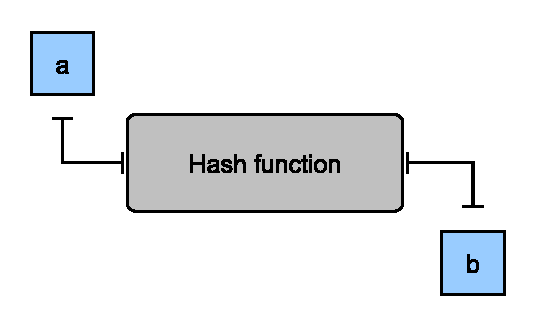
\includegraphics[width=0.6\textwidth]{hash-fn.pdf}
    \end{center}

    Al elemento $a$ que queremos guardar se le aplica la función \textit{hash} que hayamos elegido, y generará una posición que indica \textbf{dónde} debe guardarse.
\end{frame}

\begin{frame}{Representación visual}{Hash Tables}
    
    \begin{center}
        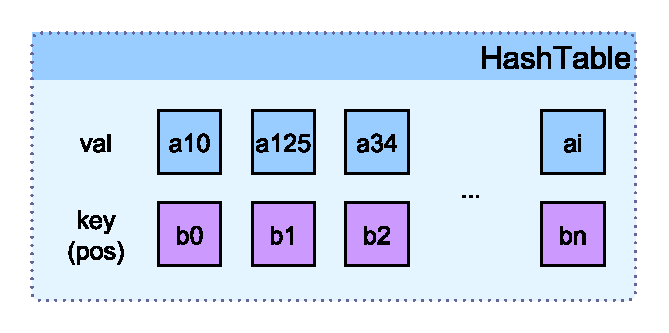
\includegraphics[width=0.6\textwidth]{hash-struct.pdf}
    \end{center}

    \begin{itemize}
        \item Al elemento ${a_{10}}$ se le aplicó una función que dio como resultado $b_0$ por lo que su lugar es el $b_0$.
        \item Al elemento ${a_{125}}$ se le aplicó la misma función y dio como resultado $b_1$ así que ése es el lugar que le corresponde\dots
        \item \dots y así para todos los elementos que queramos guardar.
    \end{itemize}

    \textit{Simple enough\dots}
\end{frame}

\begin{frame}{\dots Or is it?}{Conflictos en Hash Tables}

    Considera la función hash $h(d_1 d_2 d_3 d_4 d_5 d_6 d_7 d_8) = d_5 d_6$ que toma los dígitos quinto y sexto del valor que queremos guardar para generar una posición.

    \bigskip
    
    ¿Cuántos \textit{buckets} distintos podemos tener usando esta función hash? \pause

    \bigskip

    \begin{itemize}
        \item ¿Qué posición le toca al valor 12345678? \pause
        \item ¿Qué posición le corresponde al valor 24535655? \pause
        \item ¿Cuál le corresponde al 16895674? \pause
    \end{itemize}

    \bigskip
    
    ¡A los tres elementos les toca la misma posición!
\end{frame}

\begin{frame}{Resolución de conflictos}{Conflictos en Hash Tables}

    Hay dos opciones:

    \bigskip

    \begin{itemize}
        \itemsep3ex
        \item \textit{\alert{Open addressing}} o \textit{Rehashing} donde la estrategia es la \textbf{re-ubicación}:
        \blfootnote{\scriptsize $h$ es la función de hashing, $k$ es la llave, e $i$ es un número natural}
        \begin{itemize}
            \item \textit{Linear probing}: \quad $h(k) + i$
            \item \textit{Quadratic probing}: \quad $h(k) + i^2$
            \item \textit{Double hashing}: \quad $h_1(k) + i \cdot h_2(k)$
        \end{itemize}
        \item \textit{\alert{Chaining}} donde la estrategia es el \textbf{encadenamiento}:
        \begin{itemize}
            \item Externo: el \textit{bucket} apunta a una lista que buscamos secuencialmente para encontrar lo que buscamos
            \item Interno: el \textit{bucket} apunta directamente a otra casilla en un espacio extra designado para eso dentro de la misma tabla
        \end{itemize}
    \end{itemize}

\end{frame}

\begin{frame}
    \begin{center}
        \LARGE
        ¿Qué función debo usar?\\
        ¿Qué método de resolución de conflictos debo utilizar?\\[7ex]
        Depende\footnote{La tarea especifica qué usar. Para todo lo demás usen \texttt{std::map} {\tiny por favor}}
    \end{center}

    \begin{center}
        ¿Y los ejemplos?
    \end{center}

    \begin{itemize}
        \item Revisar las slides originales del curso
        \item Revisar el excelente material de Calvin Newton de Georgetown University
    \end{itemize}
    

\end{frame}

% \section*{Referencias}

% \begin{frame}[t]{Referencias}
    % \nocite{bibID01}
    % \nocite{bibID02}

    % \bibliographystyle{IEEE}
    % \bibliography{biblio}
% \end{frame}

\end{document}